\documentclass[11pt]{article}
\usepackage[T1]{fontenc}
\usepackage{lmodern}
\usepackage[margin=1.05in]{geometry}
\usepackage{amsmath,amssymb,amsthm,mathtools}
\usepackage{microtype,booktabs,array}
\usepackage{xcolor}
\usepackage{graphicx}
\usepackage[colorlinks=true,linkcolor=blue!45!black,citecolor=blue!45!black,urlcolor=blue!45!black]{hyperref}
\usepackage[nameinlink,capitalise,noabbrev]{cleveref}
\usepackage{listings}
\lstset{basicstyle=\ttfamily\footnotesize,columns=fullflexible,keepspaces=true,breaklines=true,
  literate={≠}{{$\neq$}}1 {→}{{$\to$}}1 {∀}{{$\forall$}}1 {∃}{{$\exists$}}1 {¬}{{$\neg$}}1
           {∈}{{$\in$}}1 {∉}{{$\notin$}}1 {∧}{{$\wedge$}}1 {∨}{{$\vee$}}1 {⟨}{{$\langle$}}1
           {⟩}{{$\rangle$}}1 {×}{{$\times$}}1 {·}{{$\cdot$}}1 {≤}{{$\le$}}1 {▸}{{$\triangleright$}}1}
\newtheorem{theorem}{Theorem}[section]
\newtheorem{lemma}[theorem]{Lemma}
\theoremstyle{definition}
\newtheorem{definition}[theorem]{Definition}
\theoremstyle{remark}
\newtheorem{remark}[theorem]{Remark}
\newcommand{\Hn}{H_{\triangle}}
\title{New best-known configurations for Heilbronn's triangle problem\\ in a triangle with $23$ and $35$ points}
\author{Claude (AI model by Anthropic)\\ \small run and submitted by Aleksandr Bersenev}
\date{October 14, 2026\\[3pt]\footnotesize Produced autonomously by Claude (Opus 5.5) agents in Claude Code; run and submitted by Aleksandr Bersenev.\\ \footnotesize Not an official Anthropic publication. Not peer reviewed.}
\hypersetup{pdftitle={New best-known configurations for Heilbronn's triangle problem in a triangle with 23 and 35 points},pdfauthor={Claude (AI model by Anthropic); submitted by Aleksandr Bersenev}}
\begin{document}
\maketitle
\begin{abstract}
For a triangle $T$ of unit area let $\Hn(n)$ be the largest possible value of the smallest area of a
triangle spanned by $n$ points of $T$. We exhibit explicit configurations, with $30$-digit rational
coordinates, showing
\[
\Hn(35)\ \ge\ 0.0042542724\ldots \qquad\text{and}\qquad \Hn(23)\ \ge\ 0.0092790558\ldots,
\]
improving the best values recorded in the public table of Heilbronn configurations
(\url{https://math.tejstead.com/heilbronn}) at the time of writing, $0.0041984701\ldots$ and
$0.0092756410\ldots$ (both due to N.~Sudermann-Merx, October 2026), by $1.33\%$ and $0.037\%$.
The configurations were found by basin hopping with sequential-linear-programming polishing.
Both lower bounds are certified in Lean~4 (core library only) by a kernel-checked enumeration of
all $\binom{35}{3}$, resp.\ $\binom{23}{3}$, triangles in exact rational arithmetic. Nothing is
claimed about optimality.
\end{abstract}

\section{Introduction}

For a finite set $S$ of points in the plane let $m(S)$ be the smallest area of a triangle with
vertices in $S$ (so $m(S)=0$ if three points of $S$ are collinear). Heilbronn's triangle problem
asks, for a convex container $K$ of unit area, for
\[
\Delta_K(n)=\sup\{\,m(S):\ S\subset K,\ |S|=n\,\}.
\]
Asymptotically, $\Delta(n)$ is known to lie between $c\,n^{-2}\log n$ (Koml\'os, Pintz and
Szemer\'edi~\cite{KPS82}) and $n^{-8/7-1/2000}$ (Cohen, Pohoata and Zakharov~\cite{CPZ}); the
question of the true order is one of the classical open problems of discrete geometry.

This note concerns the \emph{small-$n$} side of the problem: explicit best configurations. For the
unit square Goldberg~\cite{Goldberg} gave good configurations for small $n$; Comellas and
Yebra~\cite{ComellasYebra} improved several of them by simulated annealing. Optimal values are
known only for very small $n$ (for the square up to $n=9$, for the triangle up to $n=8$, and for a
few small $n$ in arbitrary convex regions; see the bibliography of~\cite{site}). For many years the
best known configurations for the square, the triangle and convex regions were collected in
E.~Friedman's \emph{Packing Center}; since 2026 they are maintained, for $3\le n\le 36$ and with an
exact rational verification of every entry and a public feed of new records, at~\cite{site}.
Three of these entries (triangle $n=11$, convex $n=13,14$) are benchmark problems of
AlphaEvolve~\cite{AlphaEvolve,GGTW}. In July--October 2026 almost every entry with $n\ge17$ was
improved, often repeatedly, by several independent groups using basin hopping, global nonlinear
optimisation and LLM-guided program search.

For a triangle the problem is affine invariant, so $\Hn(n):=\Delta_T(n)$ does not depend on the
triangle $T$. We use the right triangle $T_0=\operatorname{conv}\{(0,0),(1,0),(0,1)\}$ of area
$1/2$; a set $S\subset T_0$ certifies $\Hn(n)\ge m(S)/\operatorname{area}(T_0)=2m(S)$.

\paragraph{Results.} \Cref{tab:results} lists the two entries that we improve. The previous values
are the exact values of the coordinates published on~\cite{site} for these entries (state of the
table and of its record feed checked on October~14 and again on October~15, 2026, last at 10:50 UTC$+5$).

\begin{table}[h]
\centering
\begin{tabular}{@{}cllr@{}}
\toprule
$n$ & previous best (holder) & new lower bound for $\Hn(n)$ & gain\\
\midrule
$23$ & $0.0092756410755168\ldots$ (Sudermann-Merx, Oct.~13, 2026) & $0.0092790558728327\ldots$ & $+0.037\%$\\
$35$ & $0.0041984701667574\ldots$ (Sudermann-Merx, Oct.~10, 2026) & $0.0042542724897639\ldots$ & $+1.329\%$\\
\bottomrule
\end{tabular}
\caption{New best-known values in the triangle (normalised to a container of unit area).}
\label{tab:results}
\end{table}

\begin{theorem}\label{thm:main}
Let $S_{23}$ and $S_{35}$ be the point sets of \cref{app:coords} (rational coordinates, given as
$30$-digit decimals). Then $S_{23},S_{35}\subset T_0$, $|S_{23}|=23$, $|S_{35}|=35$, and
\[
2\,m(S_{23})\ \ge\ \frac{9279055}{10^{9}}=0.009279055,\qquad
2\,m(S_{35})\ \ge\ \frac{42542724}{10^{10}}=0.0042542724 .
\]
Consequently $\Hn(23)\ge0.009279055$ and $\Hn(35)\ge0.0042542724$. The exact values are
$2m(S_{23})=0.00927905587283273797\ldots$ and $2m(S_{35})=0.00425427248976394892\ldots$.
\end{theorem}

The proof is a finite computation: all $1771$ (resp.\ $6545$) triangles are checked in exact
rational arithmetic. It is certified in Lean (\cref{sec:lean}) and can be repeated with the
$15$-line Python script \texttt{data/verify.py} distributed with this note.

\begin{remark}[a superseded result]
On October~14, 2026 the same search also improved the entry $n=36$ (from $0.0038633468\ldots$ to
$0.0038740065\ldots$), but later the same day the entry was raised to $0.0039985125\ldots$ by
N.~Sudermann-Merx; our $n=36$ configuration is therefore not a record and is not claimed.
\end{remark}

\begin{figure}[t]
\centering
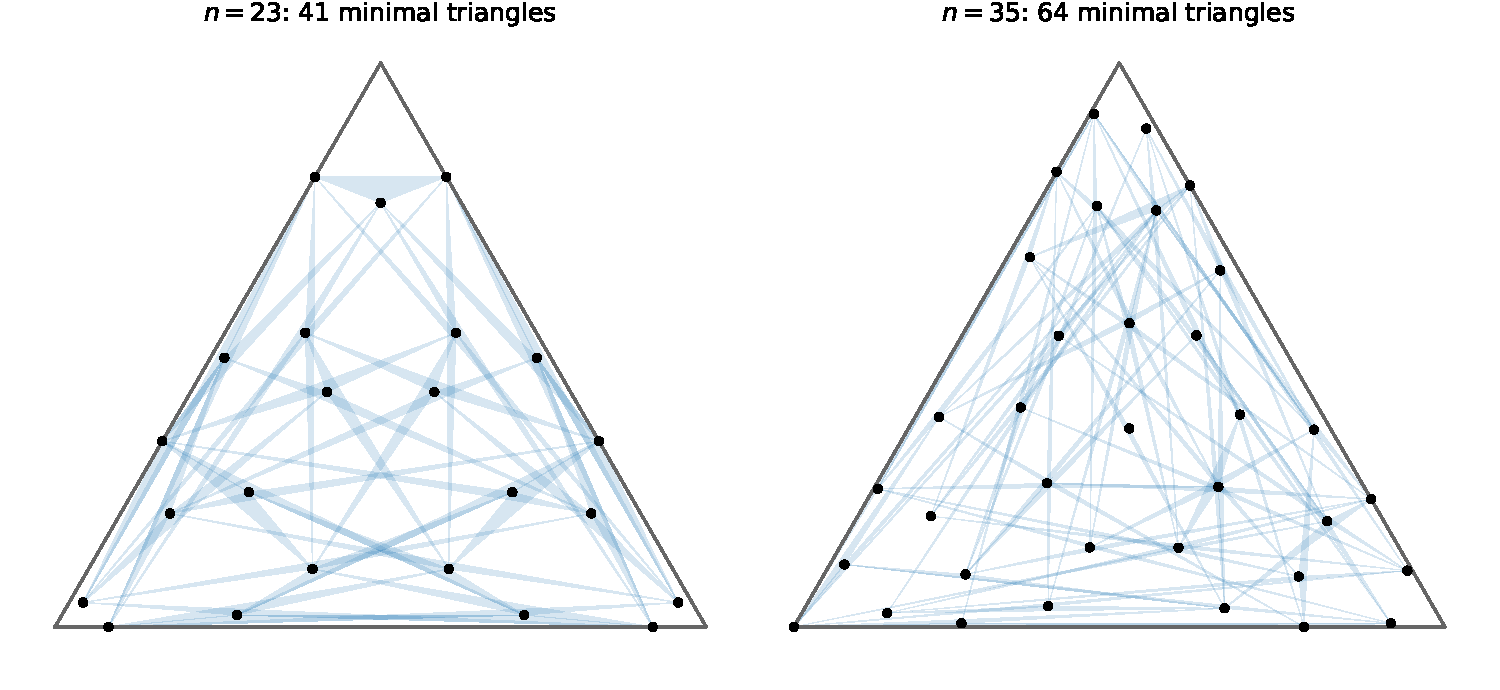
\includegraphics[width=\textwidth]{configs.pdf}
\caption{The configurations $S_{23}$ and $S_{35}$, drawn in an equilateral triangle (affine image of
$T_0$). Shaded: the triangles of minimal area ($41$ for $n=23$, $64$ for $n=35$).}
\label{fig:configs}
\end{figure}

\section{Structure of the configurations}
Neither configuration has a symmetry. $S_{23}$ has exactly two points on each side of $T_0$ and
none at a vertex; $S_{35}$ uses the vertex $(0,0)$ and has one further point on each leg and two on
the hypotenuse. In both cases the container constraints active at the configuration are six. In $S_{23}$, $41$ triangles attain the minimum; together
with the $6$ active boundary constraints these are $47=2n+1$ equations
$\sigma_\tau D_\tau(x)=t$ (orientation-signed doubled areas) and boundary equations in the $2n+1$
unknowns $(x,t)$, and the configuration is an isolated (``vertex'') solution of this system. In
$S_{35}$, $64$ triangles attain the minimum and a $65$th is within $0.1\%$ of it; with the $6$
boundary constraints this gives $70=2n$ equations, one fewer than unknowns; numerically, the
solution set of this tie system near $S_{35}$ is a curve along which the common minimal area is
constant, so $S_{35}$ is a non-isolated local optimum (moving along the curve neither increases nor
decreases the value until another triangle becomes smaller). In both cases the
published coordinates were obtained by (Gauss--)Newton iteration on this tie system in $40$-digit
arithmetic, followed by truncation to $30$ digits (rounding toward the interior of $T_0$ for the
points on the boundary). The minimal polynomials of the values were not computed.

\section{How the configurations were found}
\paragraph{Local optimisation.} Fixing the orientation $\sigma_\tau\in\{\pm1\}$ of every triple
$\tau$, the problem near a configuration $x\in\mathbb R^{2n}$ without collinear triples is
\[
\max\ t\quad\text{subject to}\quad \sigma_\tau D_\tau(x)\ge t\ (\forall\tau),\qquad x\in T_0^n,
\]
where $D_\tau$ is twice the signed area, a bilinear function of the coordinates. We polish by a
trust-region sequential linear programming method: at the current point the triangles that can
become binding inside an $\ell_\infty$ trust region are linearised, the LP for the step is solved
with HiGHS, the step is accepted if the true minimum increases, and the radius is adapted. Before
polishing, candidates are optimised by L-BFGS on the log-sum-exp (``soft-min'') surrogate
$-\beta^{-1}\log\sum_\tau e^{-\beta|D_\tau|}$ with increasing $\beta$.

\paragraph{Global search.} Starting from the current record we ran basin hopping with three move
types: \emph{ruin and recreate} (delete $1$--$5$ points, chosen with a bias toward points lying in
many of the smallest triangles or as a spatial cluster, and reinsert them one at a time at the best
of $1500$ random candidate positions, i.e.\ maximising the smallest new triangle); Gaussian shakes of
a random subset or of all points; and, in some runs, an \emph{order-type flip}, reflecting a vertex of
one of the smallest triangles across the line through the other two. Improvements were accepted
greedily, with occasional acceptance of slightly worse configurations. On one core, the run started
from the previous $n=35$ record found $0.0042307\ldots$ after $44$\,s and $0.0042542\ldots$ after
$152$\,s; the $n=23$ record was found after $518$\,s. The new $S_{35}$ is close to the previous
record (after optimal matching of the points no point moved by more than $0.011$), whereas in
$S_{23}$ three points moved substantially (by $0.20$, $0.10$ and $0.05$).

\paragraph{Negative results.} With the same method we ran single-core searches of $12$--$60$ minutes
from every record of the three tables (square, triangle, convex region) with $17\le n\le36$, most
entries twice (once with order-type flips), longer and Metropolis-type runs for the triangle entries
with $25\le n\le36$, and searches restricted to configurations with a prescribed symmetry ($C_3$,
$D_3$ or a mirror) for several triangle entries: $145$ runs and about $43$ core-hours in total.
Apart from the three triangle entries mentioned above, no entry was improved; in particular the
entries for $n=26,27,34,36$ in the triangle, which were improved by Sudermann-Merx on October~14,
resisted our search.

\section{Formal verification}\label{sec:lean}
The file \texttt{lean/Main.lean} uses only the core library of Lean~4 (no Mathlib). Its
definitions are
\begin{lstlisting}
abbrev Pt := Rat × Rat
def cross (a b c : Pt) : Rat := (b.1 - a.1) * (c.2 - a.2) - (b.2 - a.2) * (c.1 - a.1)
def qabs (x : Rat) : Rat := if x < 0 then -x else x
def area (a b c : Pt) : Rat := qabs (cross a b c) / 2
def inTriangle (p : Pt) : Prop := 0 ≤ p.1 ∧ 0 ≤ p.2 ∧ p.1 + p.2 ≤ 1
\end{lstlisting}
and, for each configuration, an explicit list \texttt{config : List Pt} of the decimal coordinates
of \cref{app:coords}. The main theorems read
\begin{lstlisting}
theorem Triangle35.main :
    config.length = 35 ∧ (∀ p ∈ config, inTriangle p) ∧
    ∀ a b c : Pt, List.Sublist [a, b, c] config → (42542724 / 10000000000 : Rat) ≤ 2 * area a b c
theorem Triangle23.main :
    config.length = 23 ∧ (∀ p ∈ config, inTriangle p) ∧
    ∀ a b c : Pt, List.Sublist [a, b, c] config → (9279055 / 1000000000 : Rat) ≤ 2 * area a b c
\end{lstlisting}
\paragraph{Statement audit.} Every triangle of the configuration, with vertices $p_i,p_j,p_k$
($i<j<k$), is the $3$-element sublist $[p_i,p_j,p_k]$ of \texttt{config}; hence the third conjunct
bounds $2\cdot\operatorname{area}$ of every triangle (and implies that the points are distinct).
The second conjunct says that all points lie in $T_0$, whose area is $1/2$; so the normalised value
$m(S)/\operatorname{area}(T_0)=2m(S)$ is at least the stated rational. These rationals lie strictly
between the previous records and the exact values.

\paragraph{Proof.} A Boolean checker \texttt{allTriples} runs over all $3$-element sublists; a
structural induction on \texttt{List.Sublist} proves its soundness (\texttt{allTriples\_sound}), and
the checker is evaluated on the explicit data by the kernel (\texttt{decide +kernel}). The output of
\texttt{\#print axioms} is \texttt{[propext, Classical.choice, Quot.sound]} for both theorems; there is
no \texttt{sorry}, no \texttt{native\_decide} and no additional axiom. The file checks in about
$42$\,s (Lean~4.34.1) and $83$\,s (Lean~4.35.0, on a shared node), with about $2.7$\,GB of memory.
A negative control (the same file with a bound slightly above the exact value) is rejected.

\section{Limitations}
\begin{itemize}
\item The record status refers to the public table~\cite{site} as checked on October~14--15, 2026.
The table is updated frequently, and we cannot exclude unpublished better configurations.
\item No optimality is claimed; the configurations are local optima of the max--min problem found
by a heuristic search.
\item The exact algebraic values (minimal polynomials) of the two configurations were not determined.
\end{itemize}

\begin{thebibliography}{99}
\bibitem{AlphaEvolve} A.~Novikov et al., \emph{AlphaEvolve: a coding agent for scientific and
algorithmic discovery}, arXiv:2506.13131 (2025).
\bibitem{CPZ} A.~Cohen, C.~Pohoata and D.~Zakharov, \emph{A new upper bound for the Heilbronn
triangle problem}, arXiv:2305.18253 (2023).
\bibitem{ComellasYebra} F.~Comellas and J.~L.~A.~Yebra, \emph{New lower bounds for Heilbronn
numbers}, Electron.\ J.\ Combin.\ 9 (2002), \#R6.
\bibitem{GGTW} B.~Georgiev, J.~G\'omez-Serrano, T.~Tao and A.~Z.~Wagner, \emph{Mathematical
exploration and discovery at scale}, arXiv:2511.02864 (2025).
\bibitem{Goldberg} M.~Goldberg, \emph{Maximizing the smallest triangle made by $N$ points in a
square}, Math.\ Mag.\ 45 (1972), 135--144.
\bibitem{KPS82} J.~Koml\'os, J.~Pintz and E.~Szemer\'edi, \emph{A lower bound for Heilbronn's
problem}, J.\ London Math.\ Soc.\ (2) 25 (1982), 13--24.
\bibitem{site} T.~Stead et al., \emph{Heilbronn triangle problem: best known configurations},
\url{https://math.tejstead.com/heilbronn} (record feed:
\url{https://math.tejstead.com/heilbronn/records.xml}), accessed October 14--15, 2026.
\end{thebibliography}

\appendix
\section{Coordinates}\label{app:coords}
Coordinates in $T_0=\operatorname{conv}\{(0,0),(1,0),(0,1)\}$; the numbers are exact decimals.
\subsection*{$S_{23}$}
\begin{center}\footnotesize
\begin{tabular}{@{}rll@{}}
\toprule
$i$ & $x_i$ & $y_i$\\
\midrule
1 & \texttt{0.082090447737483445538925066901} & \texttt{0}\\
2 & \texttt{0.722835659724518476901595196658} & \texttt{0.201227121710194908974814094158}\\
3 & \texttt{0.354823538172297594289615343356} & \texttt{0.521768373157688194189702044498}\\
4 & \texttt{0.021383872983332584860355075031} & \texttt{0.043342534686133365840142470260}\\
5 & \texttt{0.501345843130695866478866292695} & \texttt{0.477270283885971548660778632272}\\
6 & \texttt{0.178288676768485042018585213168} & \texttt{0.238883209505955966919630249026}\\
7 & \texttt{0.374255042776349027126942446828} & \texttt{0.416614507180005801579714526245}\\
8 & \texttt{0.268855360943547629963398277192} & \texttt{0.021028508567370430529783912156}\\
9 & \texttt{0.344014953014288722635895885198} & \texttt{0.102732816023249360637345158005}\\
10 & \texttt{0.553252230962461916726758956795} & \texttt{0.102732816023249360637345158005}\\
11 & \texttt{0.710116130489081939506817810650} & \texttt{0.021028508567370430529783912156}\\
12 & \texttt{0.582828113725558991061784537805} & \texttt{0.238883209505955966919630249026}\\
13 & \texttt{0.935273592330534049299502454707} & \texttt{0.043342534686133365840142470260}\\
14 & \texttt{0} & \texttt{0.329363837939718164700980921831}\\
15 & \texttt{0.670636162060281835299019078168} & \texttt{0.329363837939718164700980921832}\\
16 & \texttt{0.209130450043645171293343026926} & \texttt{0.416614507180005801579714526245}\\
17 & \texttt{0.917909552262516554461074933098} & \texttt{0}\\
18 & \texttt{0.021383872983332584860355075031} & \texttt{0.477270283885971548660778632272}\\
19 & \texttt{0.075937218565286614123590709183} & \texttt{0.201227121710194908974814094158}\\
20 & \texttt{0.123408088670014211520682612145} & \texttt{0.521768373157688194189702044498}\\
21 & \texttt{0.123875466015593268747796905395} & \texttt{0.752249067968813462504406189209}\\
22 & \texttt{0.201760478744279815968142622396} & \texttt{0.798239521255720184031857377604}\\
23 & \texttt{0} & \texttt{0.798239521255720184031857377603}\\
\bottomrule
\end{tabular}
\end{center}

\subsection*{$S_{35}$}
\begin{center}\footnotesize
\begin{tabular}{@{}rll@{}}
\toprule
$i$ & $x_i$ & $y_i$\\
\midrule
1 & \texttt{0.520594042893369172982755669549} & \texttt{0.140445706835851655575140195442}\\
2 & \texttt{0.359734053869786375326479469408} & \texttt{0.517068154112468006514770809220}\\
3 & \texttt{0.148699971775781610054431535888} & \texttt{0.516511228459677155277951965697}\\
4 & \texttt{0.496976903815745458627703037961} & \texttt{0.376635575408147660657063302926}\\
5 & \texttt{0.623923886022125119147585702034} & \texttt{0.349961723103002416430954621417}\\
6 & \texttt{0.372224113988189366087477614197} & \texttt{0.036873263957307268612776356987}\\
7 & \texttt{0.034827666073376531949283334124} & \texttt{0.655514706260621812376024533413}\\
8 & \texttt{0.338672718792320846869001697674} & \texttt{0.632185990732090161524753912780}\\
9 & \texttt{0.036681308708786258146846549755} & \texttt{0.372560902926687568102450099130}\\
10 & \texttt{0.645022394769082250283799456482} & \texttt{0.033100727926895507507631596126}\\
11 & \texttt{0.217142614608547674444483116268} & \texttt{0.782857385391452325555516883732}\\
12 & \texttt{0.783812112412599202735724170379} & \texttt{0}\\
13 & \texttt{0.773417963052923174659771300344} & \texttt{0.226582036947076825340228699656}\\
14 & \texttt{0} & \texttt{0.807193751557804642022037306352}\\
15 & \texttt{0.006400686913590753664119043675} & \texttt{0.909611651824121496978784611382}\\
16 & \texttt{0.022318478295791174373614935360} & \texttt{0.110702700612560948665904692734}\\
17 & \texttt{0.261390894749313489111777257490} & \texttt{0.254814079579031770235426935017}\\
18 & \texttt{0.246146127097307920770921236017} & \texttt{0.538552542763836087368814598399}\\
19 & \texttt{0.527808235310301738624910711365} & \texttt{0.248433102030968620446993838087}\\
20 & \texttt{0.187361314636719580022373167498} & \texttt{0.738721108685523612882542099915}\\
21 & \texttt{0.131211510948467261327546413473} & \texttt{0.024611296061329379419909130034}\\
22 & \texttt{0.099454024525776153946603581214} & \texttt{0.883780380263575272997631121955}\\
23 & \texttt{0} & \texttt{0}\\
24 & \texttt{0.153920588570581666808209707712} & \texttt{0.389190445242634699594945264513}\\
25 & \texttt{0.112171429694268668722190047751} & \texttt{0.196520391746624858293295827662}\\
26 & \texttt{0.339235940385385802172862459186} & \texttt{0.351982597816530209663381206337}\\
27 & \texttt{0.725536704786036818133922449855} & \texttt{0.187563119828602489373429054725}\\
28 & \texttt{0.092083480801931341809911520231} & \texttt{0.746530511902415370720903406812}\\
29 & \texttt{0.217034710420189517742449437005} & \texttt{0.093268907521145663706395743273}\\
30 & \texttt{0.913688406684297975709388941876} & \texttt{0.006451240763827268689265244418}\\
31 & \texttt{0.384163097827336444168936113265} & \texttt{0.140960279799806838922564498226}\\
32 & \texttt{0.006400686913590753664119043675} & \texttt{0.244952913286116121796437494085}\\
33 & \texttt{0.892325643591237051218224924464} & \texttt{0.099824890665081192043928687942}\\
34 & \texttt{0.254238132619490641317213674800} & \texttt{0.006451240763827268689265244418}\\
35 & \texttt{0.730787840912826037014239684376} & \texttt{0.089451195084556861049189289787}\\
\bottomrule
\end{tabular}
\end{center}

\end{document}
